\section{Расчеты и эксперименты}
\subsection{Собственная кривая отражения}
\subsubsection{Симметричная}

\subsubsection{Асимметричная}
Весьма наглядной иллюстрацией являются собственные кривые отражения от Si(440) рассчитанные при
трех разных углах падения и соответсвенно имею разный коэффициент асимметрии. Угол
Брегга для такой плоскости отражения составляет $\theta_B = 21.68^o$, угол наклона поверхности
составляет $\varphi = 20^o 53^{'}$.

\begin{figure}[H]
\centering
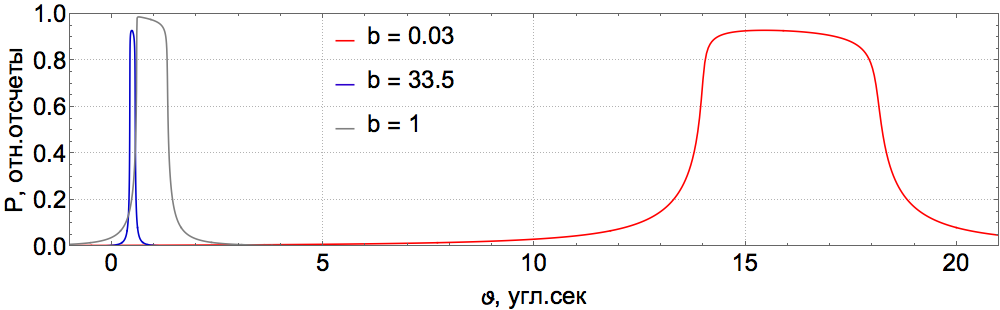
\includegraphics[width=0.99\textwidth]{images/rocking_curve_assym_3.png}
\caption{Кривые отражения 440 $MoK_{\alpha 1}$ от Si, полученные при разных углах падения(для разных b)}
\label{ris:rocking_curve_assym_3}
\end{figure}
Сдвиг центра кривой происходит из-за наличия преломления на величину 0.5 и 16.5 угловых секунд.

Варьируя угол между поверхностью кристалла и отражающей плоскостью (например, с помощью шлифовки),
можно существенно изменить ширину рентгеновского пучка (рисунок ~\ref{ris:assym_width_beam}).
\begin{figure}[H]
 \centering
 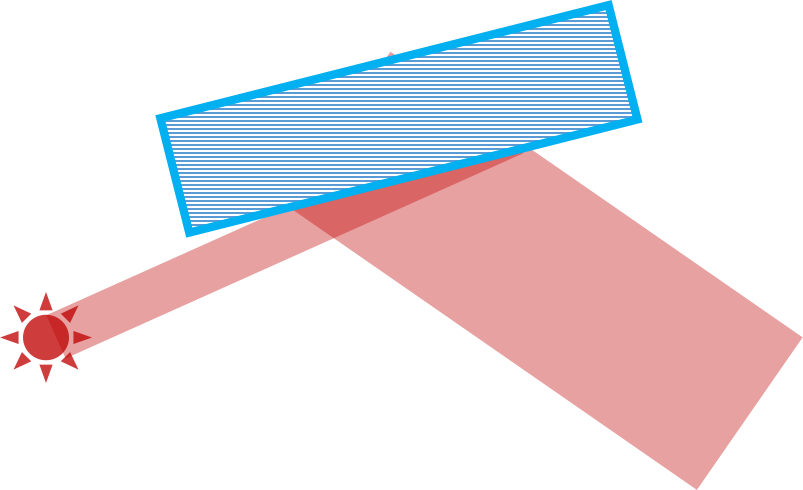
\includegraphics[width=0.4\textwidth]{images/assym_width_beam.png}
 \caption{Кристалл с асимметричным отражением по Бреггу}
 \label{ris:assym_width_beam}
\end{figure}


\subsection{Нолькристальный эксперимент}
\begin{figure}[H]
  \centering
  \subfloat[$S_1 = 20$ мкм; $S_2 = 40$ мкм;]{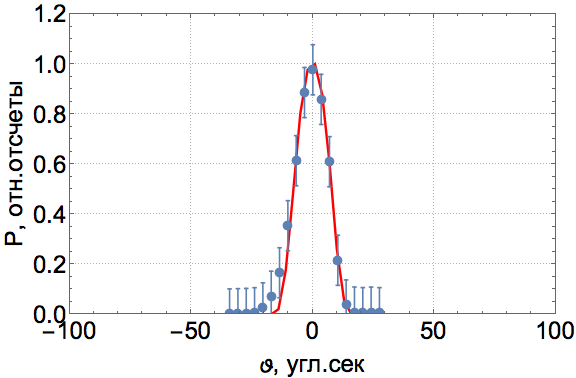
\includegraphics[width=0.3\textwidth]{images/zero_exp_20_40.png}}
  \hfill
  \subfloat[$S_1 = 40$ мкм; $S_2 = 40$ мкм;]{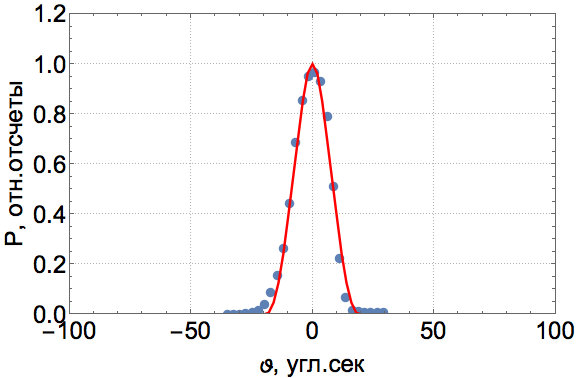
\includegraphics[width=0.3\textwidth]{images/zero_exp_40_40.png}}
  \hfill
  \subfloat[$S_1 = 50$ мкм; $S_2 = 100$ мкм;]{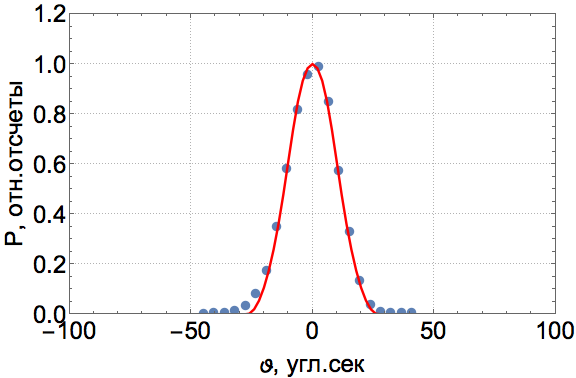
\includegraphics[width=0.3\textwidth]{images/zero_exp_50_100.png}}
  \hfill
  % \subfloat[$S_1 = 60$ мкм; $S_2 = 40$ мкм;]{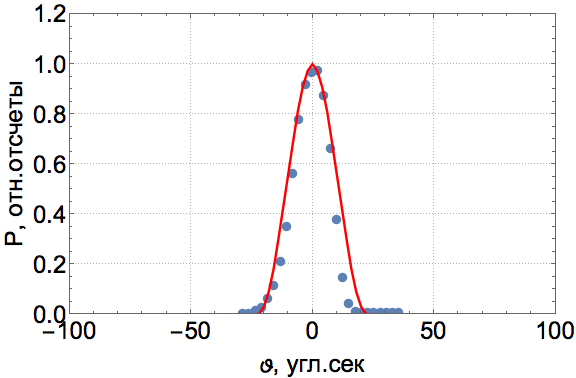
\includegraphics[width=0.3\textwidth]{images/zero_exp_60_40.png}}
  % \hfill
  \subfloat[$S_1 = 100$ мкм; $S_2 = 200$ мкм;]{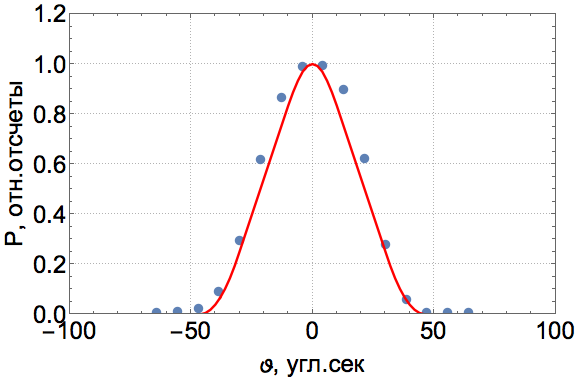
\includegraphics[width=0.3\textwidth]{images/zero_exp_100_200.png}}
  \hfill
  \subfloat[$S_1 = 100$ мкм; $S_2 = 300$ мкм;]{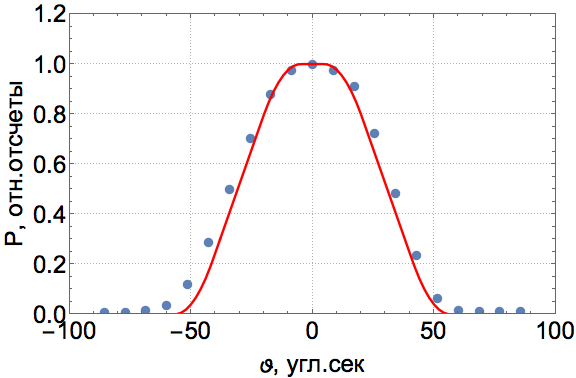
\includegraphics[width=0.3\textwidth]{images/zero_exp_100_300.png}}
  \hfill
  \subfloat[$S_1 = 200$ мкм; $S_2 = 20$ мкм;]{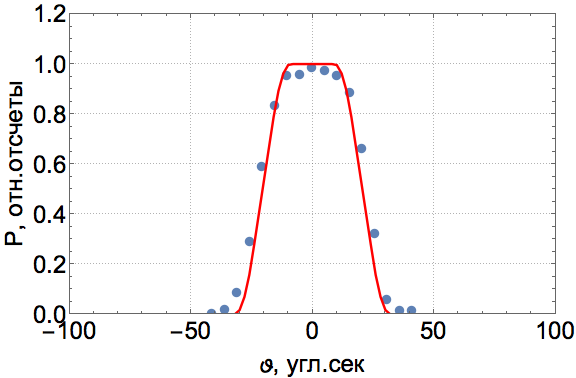
\includegraphics[width=0.3\textwidth]{images/zero_exp_200_20.png}}
  \hfill
  \subfloat[$S_1 = 200$ мкм; $S_2 = 200$ мкм;]{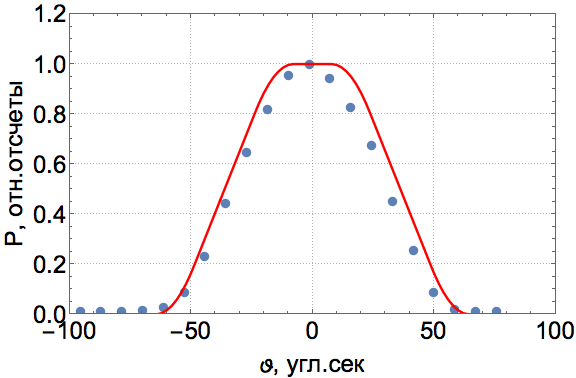
\includegraphics[width=0.3\textwidth]{images/zero_exp_200_200.png}}
  \hfill
  \subfloat[$S_1 = 200$ мкм; $S_2 = 300$ мкм;]{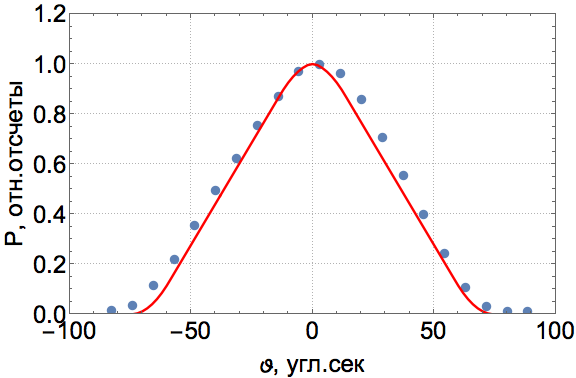
\includegraphics[width=0.3\textwidth]{images/zero_exp_200_300.png}}
  \hfill
  \subfloat[$S_1 = 300$ мкм; $S_2 = 300$ мкм;]{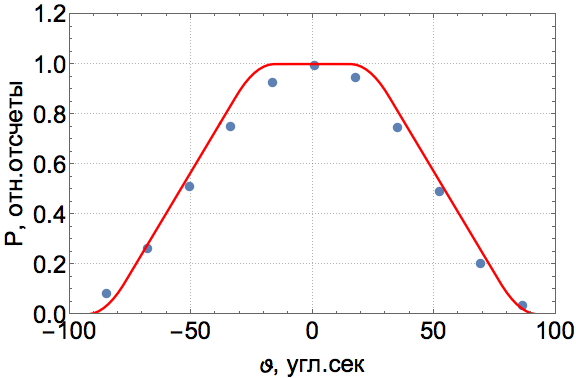
\includegraphics[width=0.3\textwidth]{images/zero_exp_300_300.png}}
  \caption{Нолькристальный эксперимент}
  \label{ris:zero_exp}
\end{figure}






\subsection{Однокристальный эксперимент}


\begin{figure}[H]
  \centering
  \subfloat[$S = 50$ мкм; ]{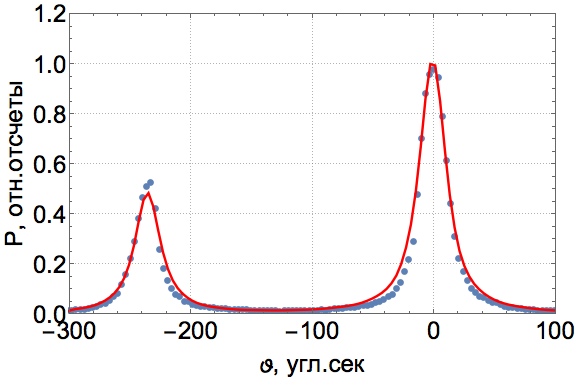
\includegraphics[width=0.7\textwidth]{images/single_cr_exp_s_005mm.png}}
  \hfill
  \subfloat[$S = 200$ мкм;]{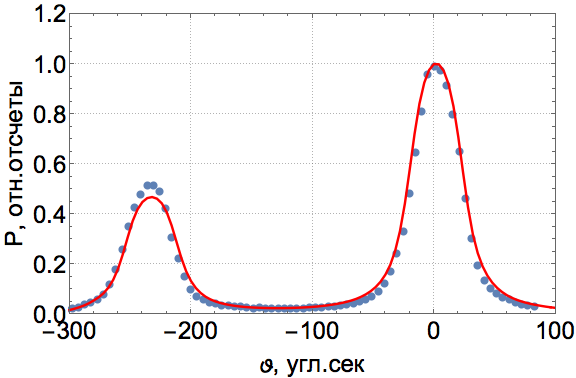
\includegraphics[width=0.7\textwidth]{images/single_cr_exp_s_02mm.png}}
  \caption{Однокристальный эксперимент}
  \label{ris:zero_exp}
\end{figure}

\subsection{Двухкристальный эксперимент}


  
\label{sec:non_disspers_KDO_section}
На рис. \ref{ris:non_disspers_kdo} приведены бездисперсионные двухкристальные КДО, рассчитанные в соответсвии
с выражением (\ref{eq:doudle_spectra_angle_map_on_detector}). В качестве кристалла-монохроматора
и образца был выбран монокристалл кремния с системой отражающих плоскостей (220), эксперимент проводился в
соответсвии со схемой, представленной на рис. \ref{ris:double_crystal_schem_lamtet_a}.

\begin{figure}[H]
  \centering
  \subfloat[]{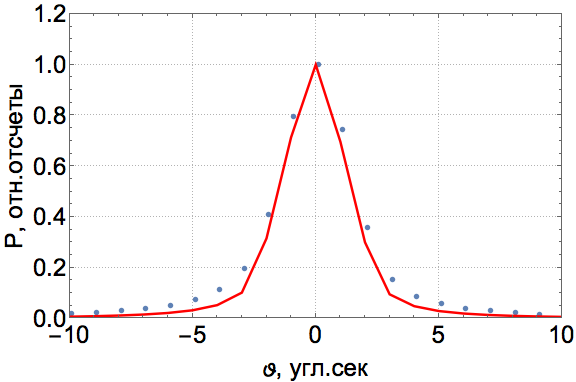
\includegraphics[width=0.45\textwidth]{images/non_disspers_20_40.png}\label{fig:f1}}
  \hfill
  \subfloat[]{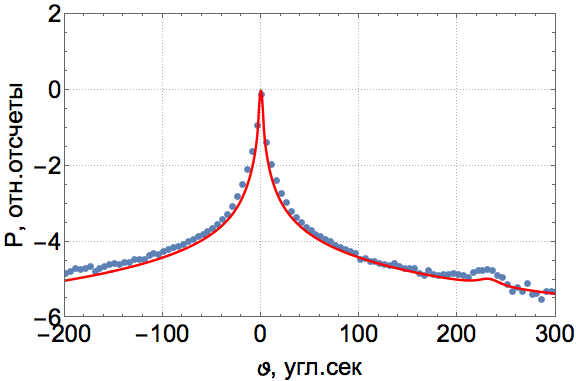
\includegraphics[width=0.45\textwidth]{images/non_disspers_20_40_log.png}\label{fig:non_disspers_kdo_1}}
  \hfill
  \subfloat[]{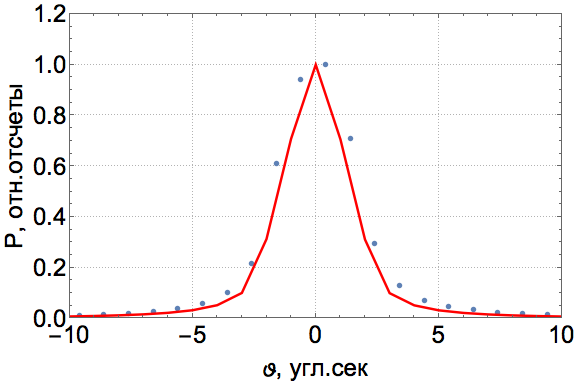
\includegraphics[width=0.45\textwidth]{images/non_disspers_300_200.png}\label{fig:f2}}
  \hfill
  \subfloat[]{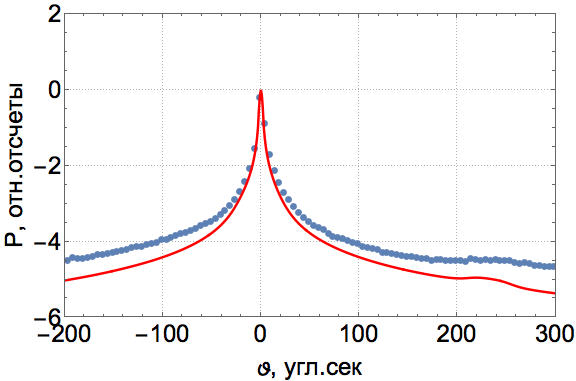
\includegraphics[width=0.45\textwidth]{images/non_disspers_300_200_log.png}\label{fig:f2}}
  \caption{Двухкристальная бездисперсионная КДО для схемы с установленными
   кристаллом-монохроматором Si(220) и образцом Si(220). Расстояние до щелевых коллиматоров
  составляет $L_1= 570 $мм, $L_2 = 1005$ мм соответсвенно.
  Линейный размер источника $\delta = 0.1$ мм. Расчет - (красная линия), эксперимент - (синие точки).
  Результаты приведены для размеров щелевых коллиматоров  $S_1 = 20 $ мкм; $ S_2 = 40$ мкм (a),
    $S_1 = 20 $ мкм; $ S_2 = 40$ мкм (b),
   $S_1 = 300 $ мкм; $ S_2 = 200$ мкм (c),
    $S_1 = 300 $ мкм; $ S_2 = 200$ мкм (d)}
  \label{ris:non_disspers_kdo}
\end{figure}

На рис. \ref{fig:non_disspers_kdo_1} видно, что наряду с главным пиком, соответствующим $K_{\alpha1}$ - линии
излучения, на которую настроен монохроматор, присутствует вклад от соседней характеристической линии
 $K_{\alpha2}$. Впервые, на это свойство двухкристальных КДО, получаемых в бездисперсионной
схеме в случае использования рентгеновской трубки было указано авторами работы \cite{chuev2008}.

\begin{figure}[H]
  \centering
  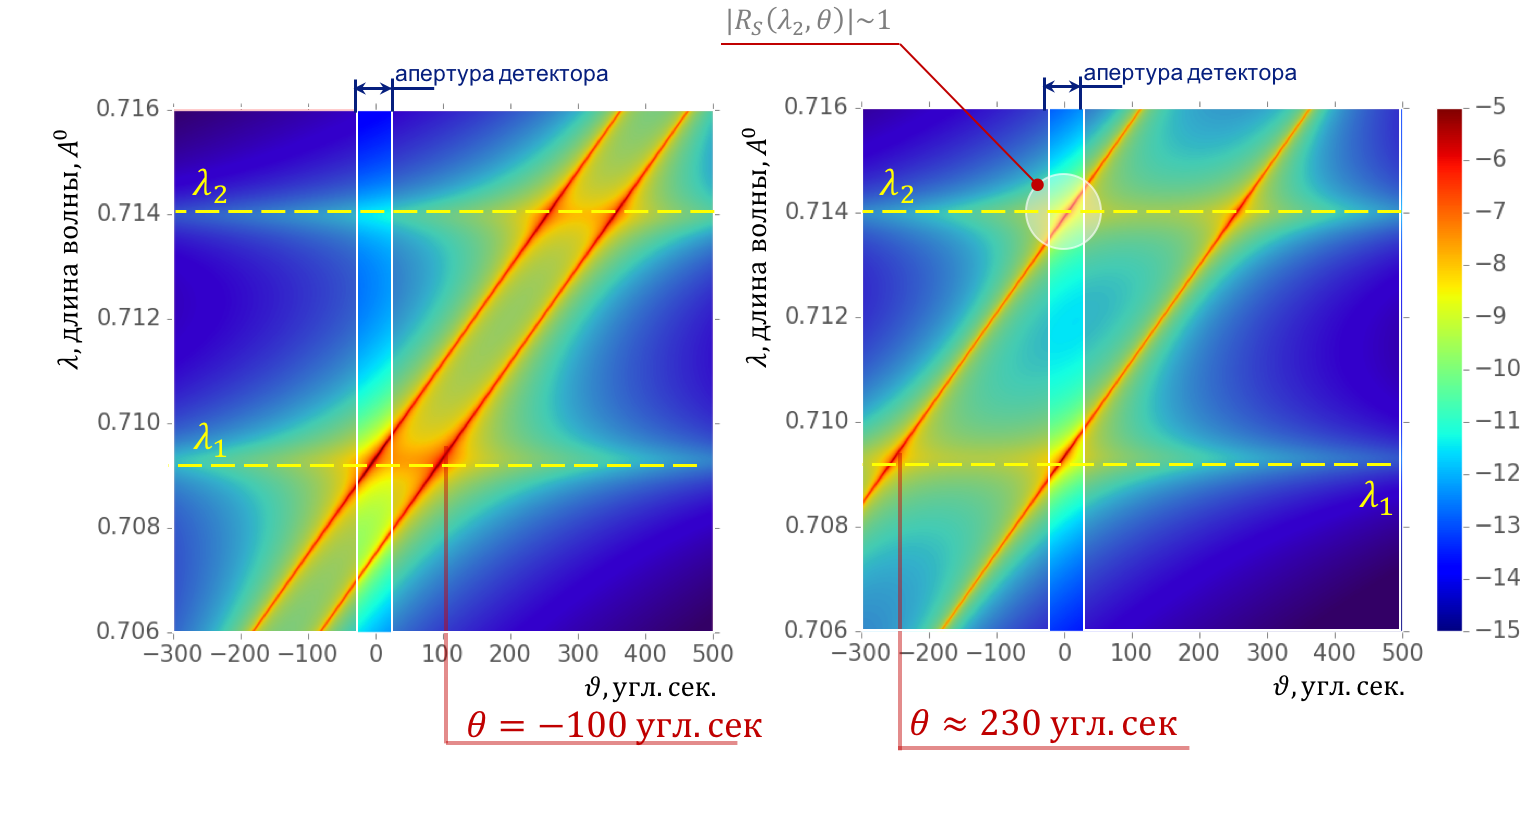
\includegraphics[width=0.8\textwidth]{images/vklad_kalpha2.png}
  \caption{Схематичное объяснение эффекта образования дополнительного пика на двухкристальных КДО
  с помощью спектрально-углового представления}
  \label{ris:vklad_kalpha2}
\end{figure}

На рис. \ref{ris:vklad_kalpha2} наглядно изображен механизм формирования дополнительного пика,
соответствующего $K_{\alpha 2}$ - составляющей спектра. В точке образования пика ($\theta = 230$ угл.сек.), коэффициент
отражения  (см. \ref{eq:doudle_spectra_angle_map_on_detector})
для кристалла образца при длине волны $\lambda_2$ максимален (в случае кристалла Si равен 1). Но отражение
от монохроматора в этой точке является слабым, т.о. интенсивность дополнительного пика на 5 порядков меньше
интенсивности основного, в отличие когда реализуется сильное отражение от обоих кристаллов.
 Необходимо отметить, что пик фактически существует вне зависимости от размера щелевых коллиматоров, но
при достаточно больших размерах (200 мкм.) пропадает на фоне хвостов КДО $K{\alpha 1}$ - линии.

  \subsubsection{Дисперсионная схема дифракции}
  Дисперсия возникает когда есть некое спектральное распределение источника и
   угол Брегга монохроматора отличается от угла Брегга исследуемого кристалла-образца
   (рисунок \ref{fig:double_crystal_schem_disp_a}).
   коэффициентом отражения.
  \begin{figure}[H]
    \centering
    \subfloat[$\theta_B^M \neq \theta_B^S$]{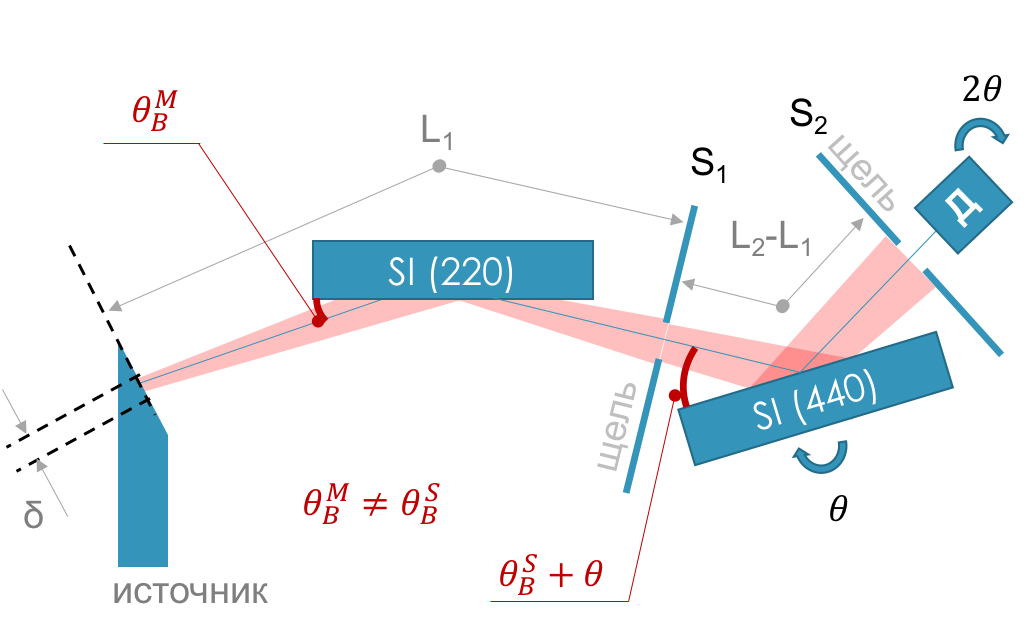
\includegraphics[width=0.6\textwidth]{images/double_crystal_schem_disp.png}\label{fig:double_crystal_schem_disp_a}}
    \hfill
    \subfloat[Спектральное-угловое распределение]{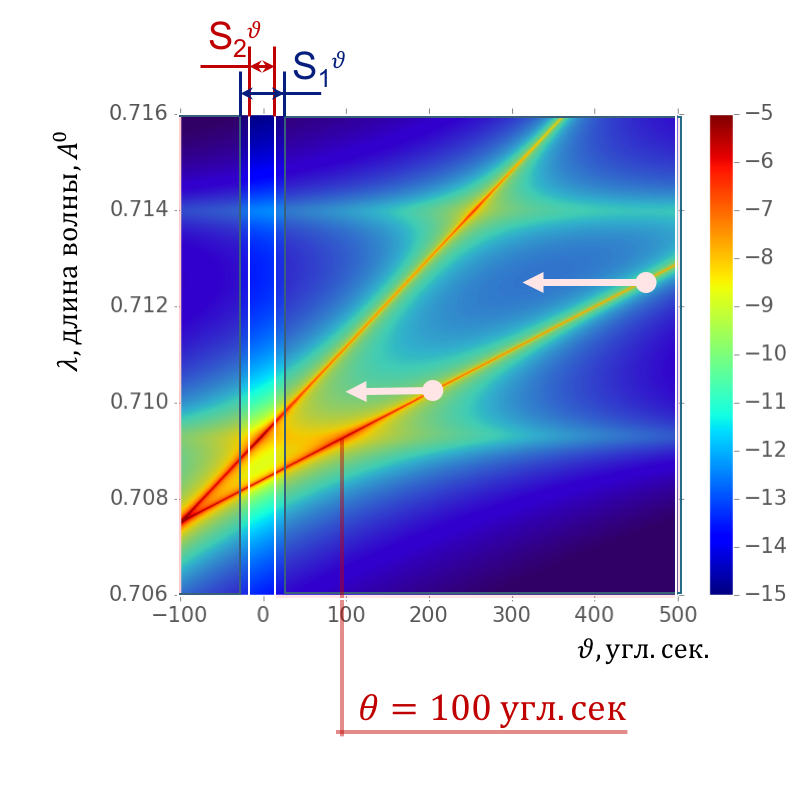
\includegraphics[width=0.35\textwidth]{images/double_crystal_lamtet_disp.png}\label{fig:double_crystal_schem_disp_b}}
    \caption{Дисперсионная схема дифракции}
    \label{ris:double_crystal_schem_disp}
  \end{figure}
  Факт наличия дисперсии возможно проанализировать на спектрально-угловом распределении
  (рисунок \ref{fig:double_crystal_schem_disp_b}), прямая образца в этом случае не параллельна прямой монохроматора и
  в области близкой к точному брегговскому отражению происходит не наложение одной на другую, как в случае отсутствия дисперсии,
  а пересечение. В точке пересечение коэффициент отражения практически равен единице,
  легко заметить что кривая отражения будет уширенной (рисунок \ref{ris:disspersion_curves_expantheory}).
\begin{figure}[H]
  \centering
  \subfloat[Образец Si(440) - $\theta_B = 21.7^o$, $S_1 = S_2 = 100$ мкм.]{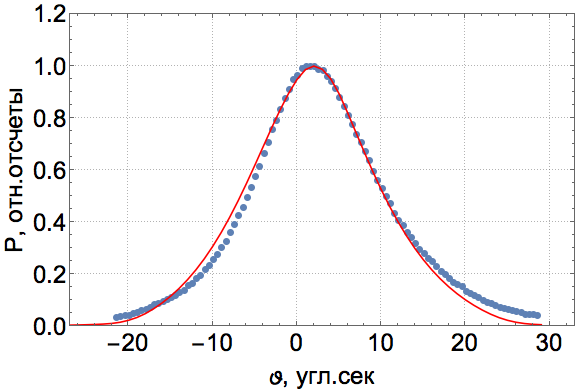
\includegraphics[width=0.45\textwidth]{images/disspers_220_440_100mcm.png}\label{fig:}}
  \hfill
  \subfloat[Образец Si(660) - $\theta_B = 33.7^o$, $S_1 = S_2 = 100$ мкм.]{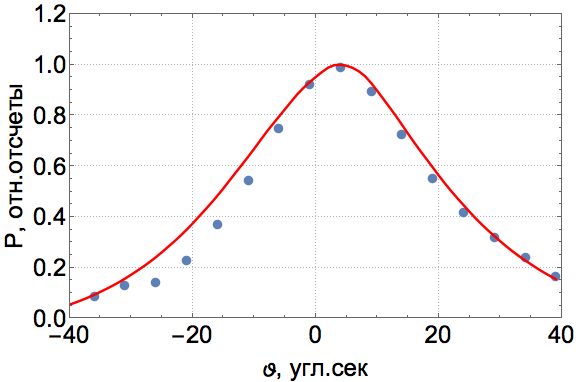
\includegraphics[width=0.45\textwidth]{images/disspers_220_660_100mcm.png}\label{fig:}}
  \hfill
  \subfloat[Образец Si(440) - $\theta_B = 21.7^o$, $S_1 = S_2 = 300$ мкм.]{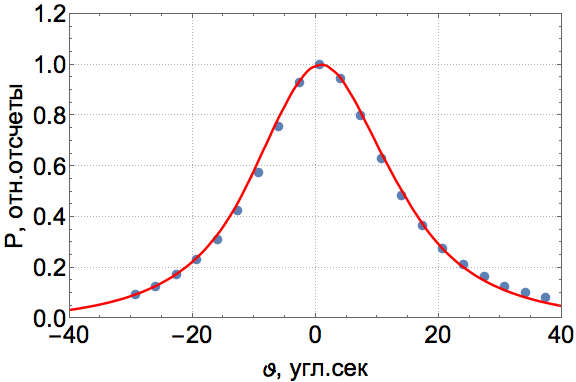
\includegraphics[width=0.45\textwidth]{images/disspers_220_440_300mcm.png}\label{fig:}}
  \hfill
  \subfloat[Образец Si(660) - $\theta_B = 33.7^o$, $S_1 = S_2 = 300$ мкм.]{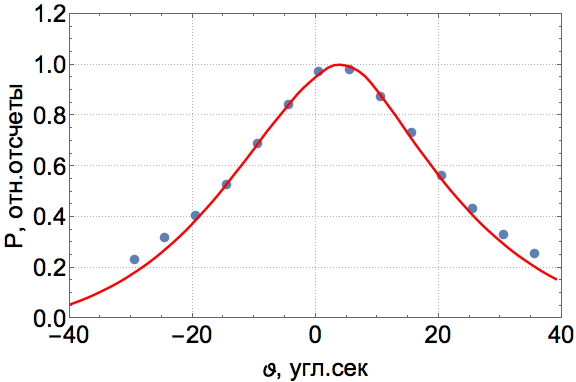
\includegraphics[width=0.45\textwidth]{images/disspers_220_660_300mcm.png}\label{fig:}}
  \caption{Двухкристальная КДО для схемы с кристаллом монохроматором Si(220) - $\theta_B = 10.6^o$ для дисперсионного случая для разных размеров щелевых устройств}
  \label{ris:disspersion_curves_expantheory}
\end{figure}

 В отличие от бездисперсионных КДО (раздел \ref{sec:non_disspers_KDO_section}) заметно присутствует
 влияние размера щелевых устройств.

    \subsubsection{Асимметричная схема дифракции}


  \begin{figure}[H]
    \centering
    \subfloat[$b = 33.52$, $\varphi$ > 0]{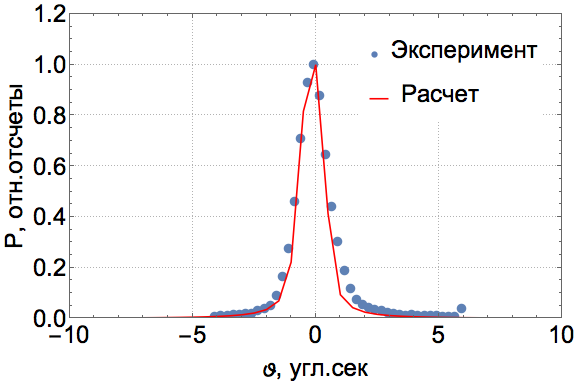
\includegraphics[width=0.45\textwidth]{images/assym-blue-50.png}}
    \hfill
    \subfloat[$b = 0.03$, $\varphi$ < 0]{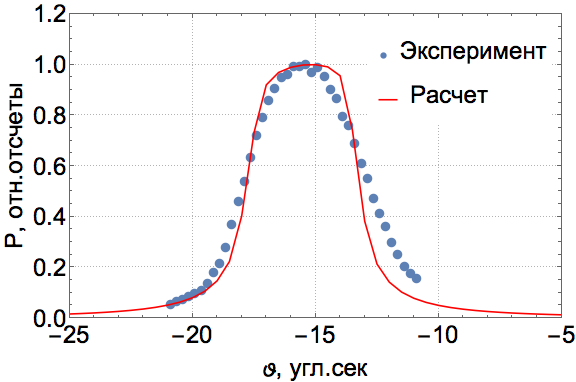
\includegraphics[width=0.45\textwidth]{images/assym-red-50.png}}
    \caption{Двухкристальная КДО для схемы с кристаллом монохроматором Si(440) и асимметричным образцом Si(440),
    угол разориентации поверхности $\varphi = 20^o53^{'}$. Размер щелевых устройств $S_1 = S_2 = 50$ мкм.}
    \label{ris:assymetric_exp_50}
  \end{figure}

